\section{Conclusions} \label{sec:conclusions}
In this section I will compare the results of the AlexNet with learning rates of 0.0001 and the CNN with learning rates of 0.001 since they have the best results.
As we can see in Figure~\ref{fig:accuracy} and Figure~\ref{fig:loss} both the models have similar results but the CNN seeems to converge faster than the AlexNet.

However the dataset is not big enough to train a deep neural network and the results are not very good.
In fact also training for more epochs the model does not improve the results because the model starts to overfit the training data.

\begin{figure}[h]
    \centering
    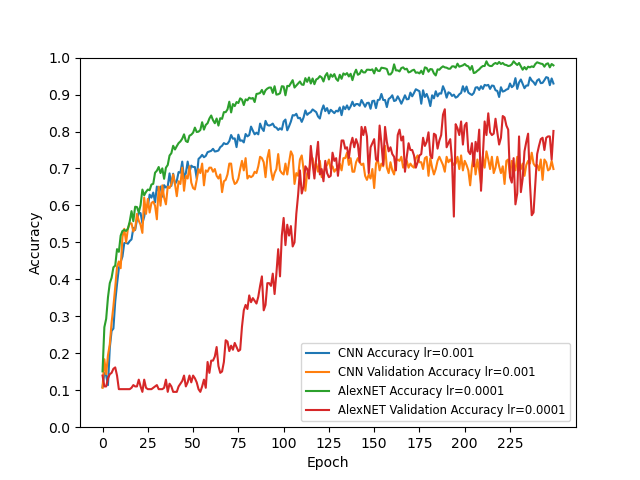
\includegraphics[width=0.5\textwidth]{../plot/accuracy.png}
    \caption{Training and validation accuracy for the AlexNet and the CNN}\label{fig:accuracy}
\end{figure}

\begin{figure}[h]
    \centering
    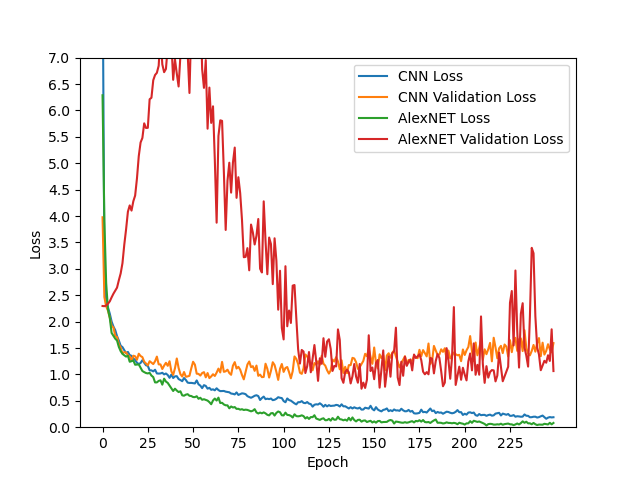
\includegraphics[width=0.5\textwidth]{../plot/loss.png}
    \caption{Training and validation loss for the AlexNet and the CNN}\label{fig:loss}
\end{figure}